

\begin{figure}[t]
    \centering
    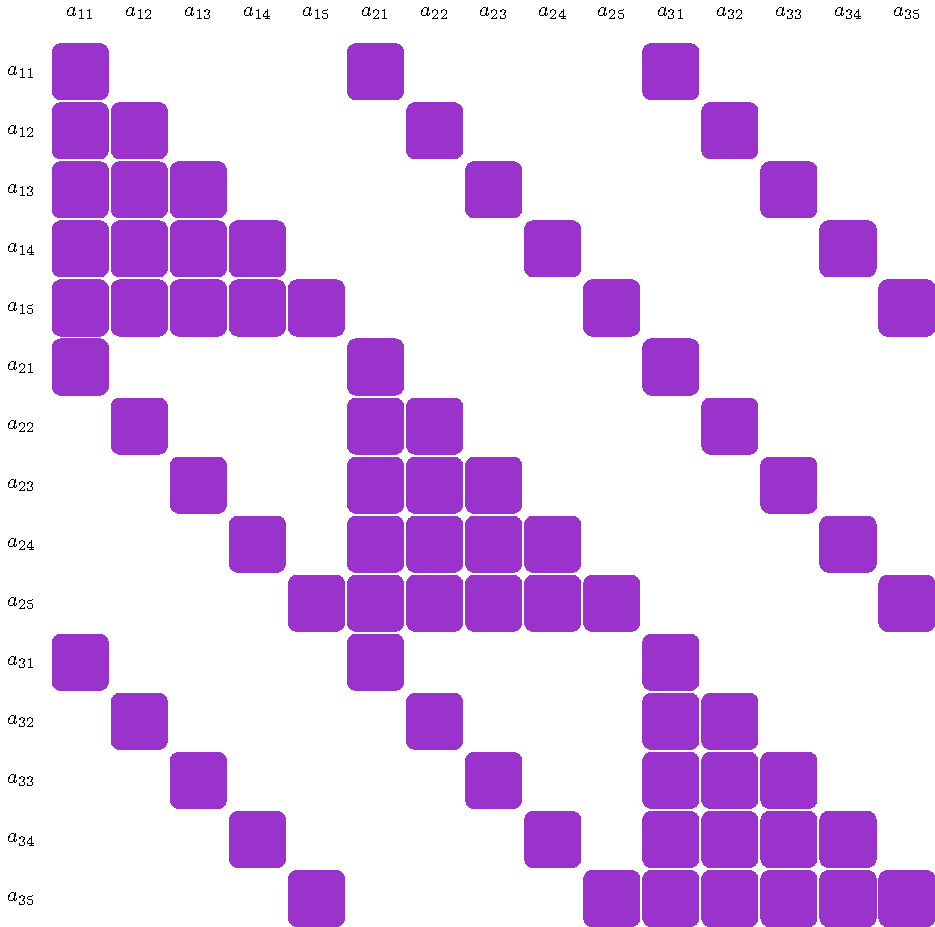
\includegraphics[width=.45\textwidth]{figs/attention.pdf} 
    \caption{Attention matrix for the world model.}
    \label{fig:apx:attention}
\end{figure}

\begin{figure}[t]
    \centering
    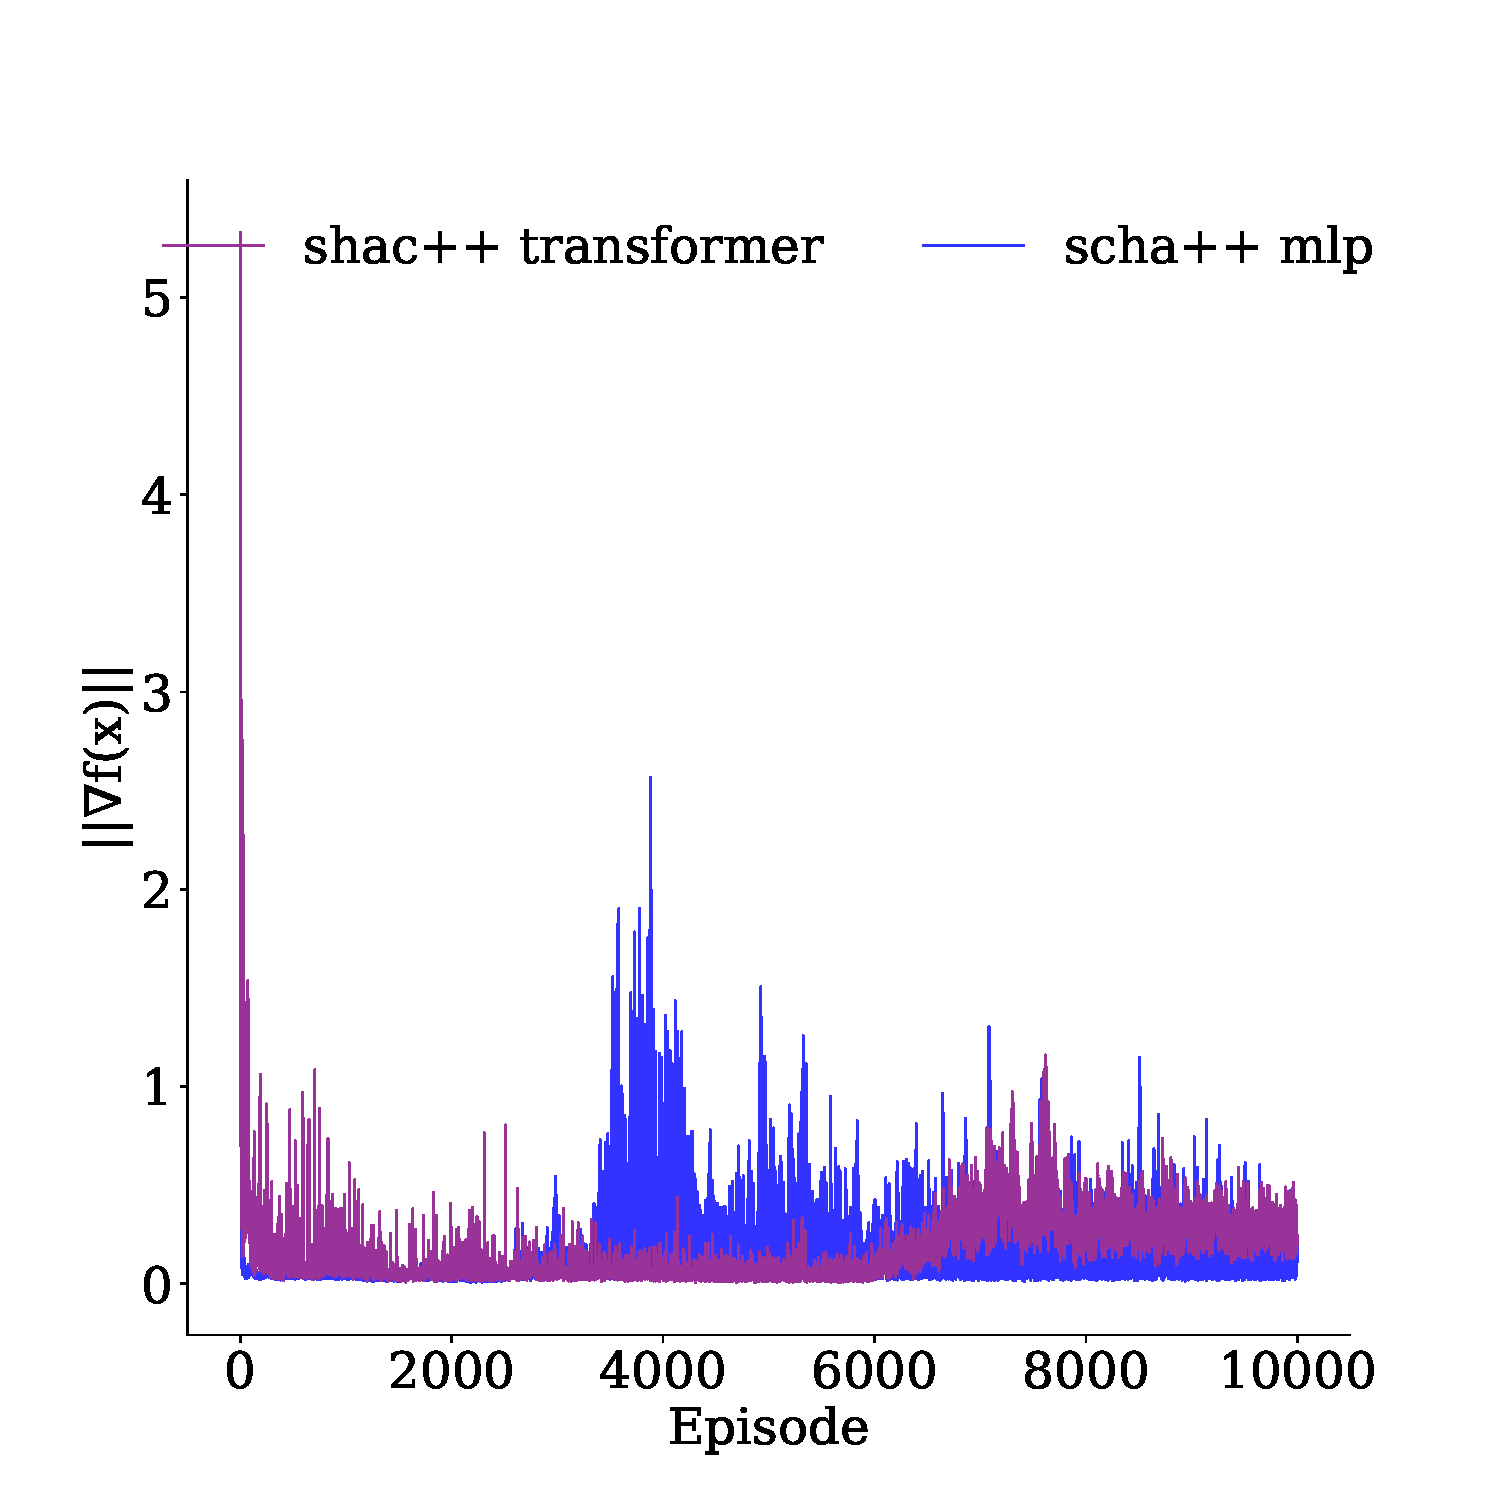
\includegraphics[width=.45\textwidth]{figs/grads-mlp-transport.pdf}
    \caption{Gradient norm for a transformer architecture wrt. a MLP architecture.}
    \label{fig:grads-mlp}
\end{figure}


\section{Architectures}\label{apx:arch}

As mentioned earlier, we test PPO, SHAC, \fname{}, and \fnamer{} with two different architecture---Transformer and MLP. The former is a popular positional invariant architecture for sequence modeling~\cite{Vaswani17}. While the latter is a simple feed-forward neural network.

The main advantage of the transformer architecture is its positional invariance property. In fact, the order in which the agent's observation are fed into the network should not affect the ultimate outcome, at least, for the tested environments. We believe that this leads to better sample efficiency that it is ultimately observed in policies achieving higher rewards (see \Cref{tab:max-rewards}). 

In contrast, the MLP is fed with a concatenation of all agent observations. This results in a simple and lightweight implementation, leading to faster inference times. However, in our experiments, the MLP appears to underperform compared to the transformer architecture.

\subsection{Policy/Value/Reward MLP Network}
When implementing the policy, value, and reward functions with an MLP, we use a single hidden layer with sizes of $32$, $96$, and $160$, depending on the number of agents. This choice was made to account for the increasing complexity that a higher number of agents should introduce. The activation function is always ReLU, and dropout is used only for the policy network. The learning rate is consistently set to $0.001$. The cache for training these networks is set to $30,000$ samples. Gradient clipping is applied only to the policy network, with a threshold of $1$. For a full list of hyperparameters, see \Cref{apx:tab:shac} and \Cref{apx:tab:ppo}.

\subsection{Policy/Value/Reward Transformer Network}
When implementing the policy, value, and reward functions with a transformer, we use a single hidden layer with a size of $64$, regardless of the number of agents, and a feed-forward size of $128$. We do not scale these sizes with the number of agents, as the transformer is expected to natively scale with the sequence length. The remaining hyperparameters are set consistently with those used in the MLP architecture. For a full list of hyperparameters, see \Cref{apx:tab:shac} and \Cref{apx:tab:ppo}.


\subsection{World Model}
When implementing the action world model, we consistently use a transformer architecture. Each action is represented as an embedding fed into the network. To maintain positional invariance between the agents, we employ a custom attention matrix that allows the action for step $i$ of agent $j$, $a_{ij}$, to attend only to actions from the same step or previous steps of the same agent. Formally, $a_{ij}$ can attend to all $a_{kj}$ for $k<i$ and to all $a_{ik}$ for $k \in \agents$. This attention pattern is shown in \Cref{apx:fig:attention}. As a result, the world models process sequences of length $32 \cdot \na$. We use a slightly deeper architecture to account for the increased complexity of the task, with $3$ layers. The hidden size is set to $64$ and the feed-forward size to $128$. The remaining hyperparameters are set consistently with those used in the MLP architecture. For a full list of hyperparameters, see \Cref{apx:tab:shac}.

